\documentclass[journal]{IEEEtran}

\usepackage{cite}
\usepackage{amsmath}
\usepackage{verbatim}
\usepackage{multirow}
\usepackage[unicode,pdftex]{hyperref}
\usepackage{xcolor}

\ifCLASSINFOpdf
\usepackage[pdftex]{graphicx}
\else
\fi

\usepackage{todonotes} 
\hyphenation{op-tical net-works semi-conduc-tor}

\newcommand{\reffig}[1]{Fig. \ref{#1}}
\newcommand{\refsec}[1]{Section \ref{#1}}
\newcommand{\refeq}[1]{Eq. \ref{#1}}
\newcommand{\reftab}[1]{Table \ref{#1}}

\newcommand{\tabincell}[2]{\begin{tabular}{@{}#1@{}}#2\end{tabular}}
\newcommand{\stodo}[1]{\todo[size=\tiny]{#1}}


\DeclareMathOperator*{\argmax}{argmax}
\DeclareMathOperator*{\argmin}{argmin}


\definecolor{level2}{RGB}{255,255,255}
\definecolor{level3}{RGB}{10,10,10}
\definecolor{revised}{RGB}{100,101,140}
\definecolor{continue}{RGB}{255,0,0}
\definecolor{filltext}{RGB}{0,255,255}

\begin{document}
\title{Background Subtraction via Deep Variation Transformation}

\author{Yongxin Ge, 
        Xinyu Ren, 
        Chenqiu Zhao}

% XXX there is no such command of authorruning!!!!!!
% XXX 根本就没有authorruning 命令!!!
% \authorrunning{Lecture Notes in Computer Science: Chongqing University}


\maketitle



\begin{abstract}
%
Previous approaches to background subtraction generally analyzes the variation of pixels' observation.
%for background subtraction.
%
%Background subtraction is generally considered as the binary classification of pixels' observations in time sequence,
%and preivous work 
%
%Previous work analyzes the variation of pixels for background subtraction which is generally considered as the binary classification of pixels in time sequence.
%
%
In this paper, we focus on transforming the variation into a new space where that there is an obvious difference between the patterns of variation produced by the moving objects and the background,
and a novel background subtraction method called Deep Pixel Variation Transformation Learning (DPVTL) is proposed.
%
% 
%     
%     
%     another space where the observations of pixels are easier classified,
% with the motivation to  that there is difference between the patterns of variation produced by the moving objects and the background.
% %
% We also put forward a novel background subtraction method called Deep Pixel Variation Transformation Learning (DPVTL) is proposed.
% %
% with the consideration that the observations of pixels are usually so hard to analyze due to the unpredictability and complexity of natural scenes,
%and a novel background subtraction method called Deep Pixel Variation Transformation Learning (DPVTL) is proposed.
%
In particular,
the variation is represented by the sequence of pixels' observations and used as the input of the fully convolutional network.
%
Then, the fully convolutional network is trained to learn the pattern of variation for the transformation followed by a liner classifier for labeling the pixels as foreground or background.
%    with the supervision leaded by grounthtruth data.
% XXX 这句话还是有点问题
Benefied from the ingenious utilization of deep learning network leading by our clear congnition of essence about background subtractoin problem,
proposed approached adaptively generate superior peroformances in diversly complex scenes.
%
Comprehensive experiments in standard benchmarks demonstrate the superiority of proposed approach compared with state-of-the-art methods including both deep learning and traditional methods.
%
% We also put
% forward a novel background subtraction framework called the
% Integration of Foreground and Background (IFB) cues.
% % a video stream. 
% %之前方法 下一句用的focus on加ing,这就用ed,形成对比
% % Previous works generally proposed the artificial model with the utilization of lowlevel or hand-crafted features to analyze the variation of pixels' observation.
% Previous work generally analyze the variation of pixels' observation with the u/cygdrive/c/Users/Ray/Downloads/3.iebktilization of hand-crafted features.
%     %in time sequence.
% % 为什么之前方法会失败
% However, due to the complexity and diversity of nature,
% the variation of observations becomes so hard to classify by hand-crafted features.
%     %in complexly natural scenes.
% %我们的改进
% In this paper, we focus on transforming the obserations sequence into another easier classfied space,
% and a novel background subtraction method based on Deep Variation Transformation (DVT) is proposed.
% % XXX 为什么是networks,不是network呢?
% In the DVT model,
% the fully convolutional network (FCN) is untlized to transform the sequence of pixels' observations into a new representation of pixels' observations with more obvious features for classfication.
% %
% In particlar, 
% a the variation of observation represented by pixel sequence is reshaped into a image patch as the input of FCN network.
% %
% Then, the output of network is classfied and reverted to the corresponding sequence for the binary classfication of oberservations' variation.
% %
% Benefied from the ingenious utilization of FCN network leading by our clear congnition of essence about background subtractoin problem,
% proposed approached adaptively generate superior peroformances in diversly complex scenes.
% %
% Comprehensive experiments in standard benchmarks demonstrate the superiority of proposed approach compared with state-of-the-art methods including both deep learning and traditional methods.
% 
% 
% 
% videos are divided into fixed length image stacks by temporal sampling. 
%     Next, image stacks is broken down into pixel observation matrixes as the input of the FCN to learn the patterns of pixel variation. 
%     Each of the pixel matrixes contains a piece of temporal information about pixel variation over a period of time.  
% The architecture of our FCN is devised from the semantic segmentation problem. 
% %效果
% Experiment shows that our model has a strong learning ability to the patterns of those permutations of pixels’ observations. 
%     Compared with some state-of-the-art methods, both deep learning and traditional methods, the proposed approach outperform its conventional counterparts significantly owing to the utilizing of temporal information.
\end{abstract}

\begin{IEEEkeywords} 
    Background Subtraction, Feature Transformation, Deep Learning,
\end{IEEEkeywords}

\IEEEpeerreviewmaketitle

\section{Introduction}
%背景检测的背景介绍
Background subtraction as a fundamental problem in computer vision\ \cite{Bouwmans201431} has been discussed over decades with the increasing number of cameras,
which is widely used as the pre-processing step of video processing \cite{Barnich2011_2011_TIP}.
% which can help us efficiently mark the region of interest,
% thus saving us huge amount of computing resources\ \cite{Barnich2011_2011_TIP}.
%\todo{cited an article to support this sentence.}
% 现有的方法在简单场景中效果很好了
Existed methods have already achieved well performances in the scenes of low diversity or complexity, such as the indoor scenes.
However, it still remains a challenging problem in the scenes with high complexity and diversity.
% 传统的方法是怎么做的,有什么问题
Traditioanlly, background subtraction algorithms focus on anaylsing the pixels' variation for background subtraction,
since the background subtraction is typically recognized as a binary classification that assigns each pixel in a video sequence with a label, 
for either belonging to the background or foreground scene.
% 总而言之,background subtraction依然有很多问题
However, due to the unpredictability and complexity of the pixels' variation in natural scenes,
the variation becomes so unordered which is hard to be analyzed for background subtraction.

% 第二段重点阐述什么是deep variation learning
% 在多样的自然场景中,前景可能产生和背景相似,甚至相同的像素,而这种像素很难去分析
In the diversely natural scenes,
it is possible that the moving objects produce the similar or even the same observations of pixels to that of background,
and the variation of observations becomes so hard to analyze when it includes such observations.
% similar to their counterparts of background but atually belong to foreground .
% 如图所示,像素观测值C就和背景的值几乎一模一样,
As shown in the \reffig{idea},
the observation C is closely related to the observations belong to the background but it is actually produced by moving objects and should be classified as foreground.
% 大多数情况下,他都会被划分成背景
However, in most cases, it is highly possible that the observation C will be falsely classified as background by previous work due to the similarity with their counterparts of background.
% 我们的就是希望把这个variation 转化到更简单的地方去
In this work, we focus on transforming the variation of pixels' observation into a new variation where the observations are easier to classified,
as shown in the bottom part of the \reffig{idea},
with the motivation that the pattern of fragment consist of observations A-D can be learned by the network and transformed into another fragment where these observations are easily and correctly classified as foreground.
% transformatin 之后,就很容易分类了,然后这就是我们的方法的核心了
Based on this motivation, the Deep Variation Transformation model for background subtraction is proposed.
% 
% %实际应用中的挑战
% \todo{the main purpose of the second paragraph is showing our idea. But be careful that you should not mention any details of our method which is the content of third paragraph. Pls re-write this part according to figure 1. The main content should be the description of figure 1, as well as our idea, insight}
% Existed methods have already achieved well performances in the scenes of low diversity or complexity, such as the indoor scenes. 
% However, background subtraction is still unsolved because of the complexity and the diversity of natural scenes.
% There are many forms of natrual scenes, for example, camera jitter, dynamic background, bad weather, illumination changing, intermittent object motion\cite{CDN2014}. In these situations, the backgrounds are no longer being static, while in fact, the background can be dynamic and complex, which brings some severe challenges to the traditional methods.
% To solve this problem, we bring up a novel conception of variation transformation, wherein the historical observations of each pixel are conceived as a unity, the pixel variation. Each piece of pixel variation contains the complete temporal information of historical observations, which turns out to be our advantage that not only the distribution of observations, but also the temporal coherence plays an important role in the task.
\begin{figure}[!t]	% FIGURE: figure/fig1 
\centering
    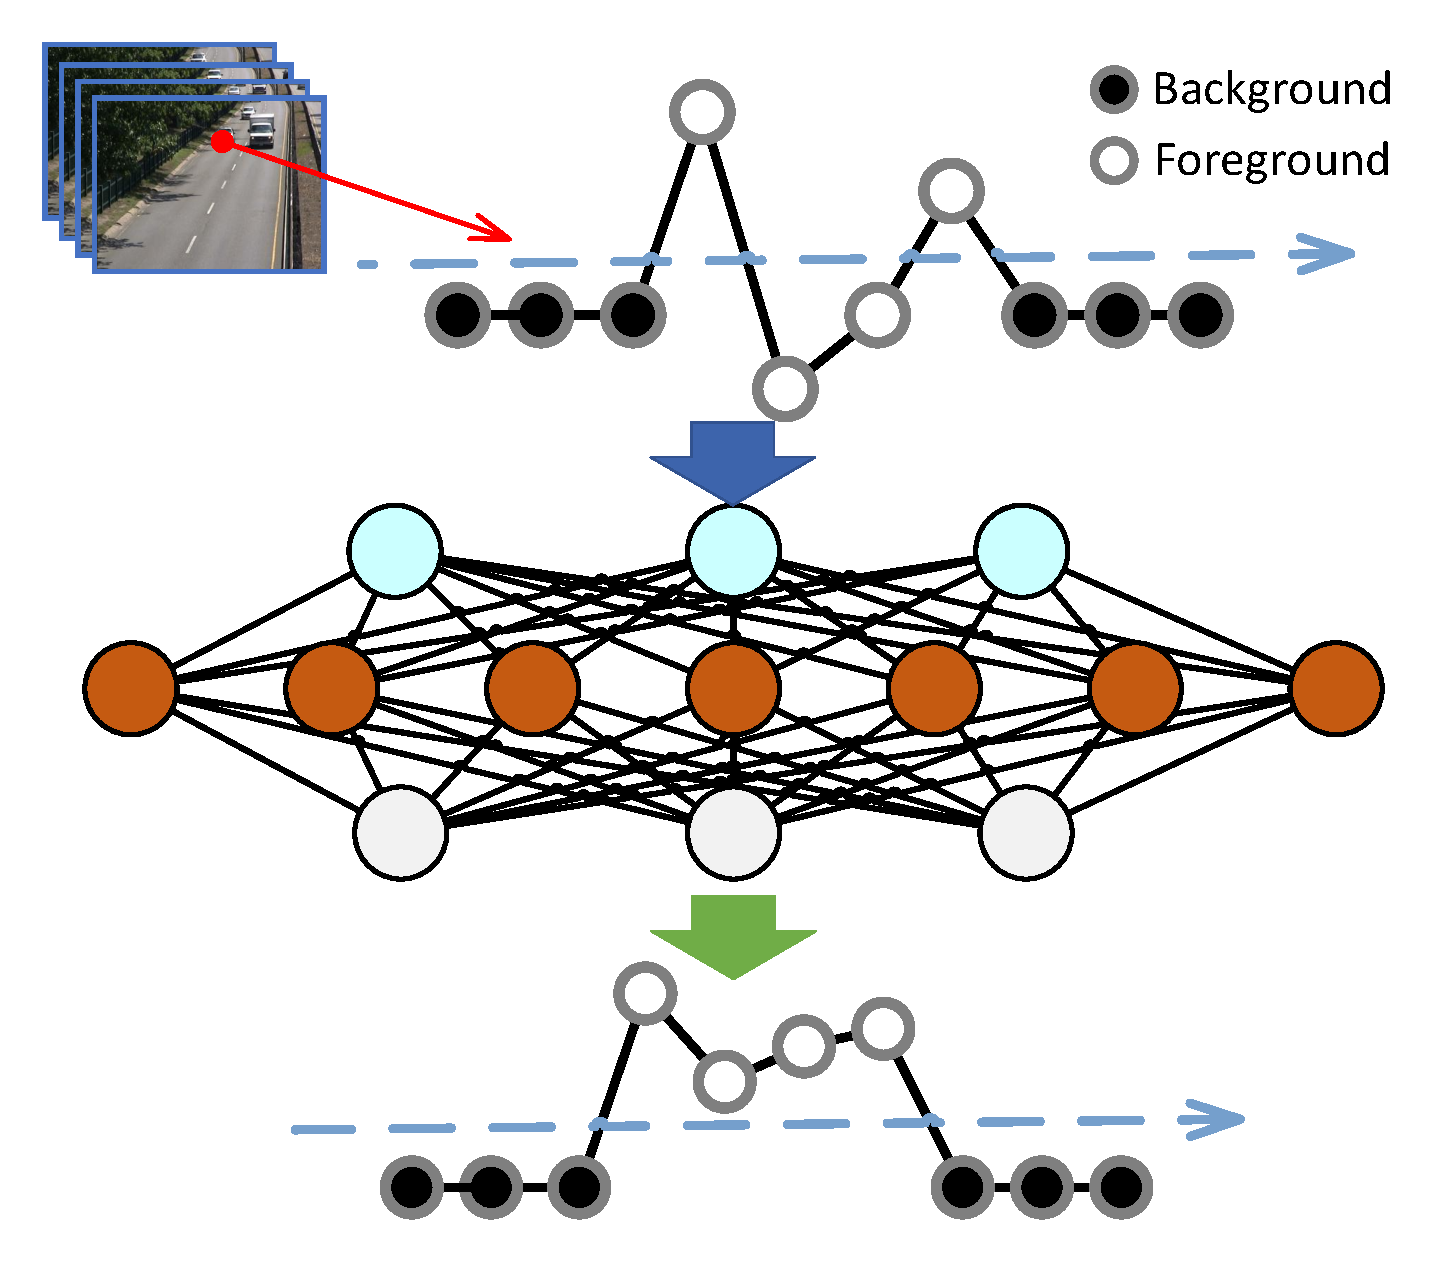
\includegraphics[width=\linewidth]{figure/demo.pdf}
    % 图例里描述一下。
    \caption{The demonstration of deep variation transformation. Due to the complexity of natural scenes, the original pixels' variation is hard to classify correctly. After transforming by deep learning network, the pixels in variation become easy to be classified as foreground and background correctly.}
    \label{idea}
\end{figure}

%本文的想法和优势
% The previous methods have already made great progress in generating some sophisticated background models with given videos. 
% Unfortunately, some instructive clues have been long put aside and neglected, since there is no efficient way to deal with them. 
% For instance, the statistical methods\cite{Stauffer1999} model the pixel-wise distribution of historical observations over time, while having no concerns over the sequential information in a video stream. 

%具体介绍
% XXX 一句话,换一行!!!
% In this paper, we propose a novel Deep Variation Transformation Learning (DVTL) model for background subtraction in diversely natural scenes. 
In the DVTL model, 
the sequence of pixel observations is used to represent the variation and input into the network for learning,
which encode both the intensity distribution and sequential information.
%
Then, a Fully Convolutional Network (FCN)\ \cite{Shelhamer2017fcn} is applied to learn the patterns of the pixel variation and find a transformation which guarantee the linear separability of transformed pixel variation generated by mapping in a new space.
%
In particular,
we take advantage of the strong learning ability of FCN to learn an end-to-end representation of the pixel variation in a new space where they can be easily classified to background and foreground.
%
Benefited from the strong learning ability of FCN,
proposed approach works well in diversely complex scenes adaptively.
%
%Moreover,
%since the pixel sequences are extracted from individual pixels, a large number of pixel matrixes may be extracted from only a single image stack, which promises that sufficient training data can be obtained with limited groundtruth.
% 
% 
% 
% \todo{This paragraph is too short! provide comprehensive details of our work!}
% % The final prediction can be obtained by thresholding of the transformed variation. 
% %Our contributions can be summarized as follows:
% The contridbutions of proposed approach are shown as follows:
% \begin{itemize}
% \item We proposed the pixel observation matrix to describe the pixel variation, which encode both the intensity distribution and sequential information over time.
%     The observation matrix is obtained by reshaping the vector of a pixel's historical observations, subtracted from the image stacks. 
% \item We propose a deep neural network for variation transformation. 
%     Our FCN network is trained to learn the pixel variation and generate a new representation in a new feature space. 
% \end{itemize}
% 
%文章结构

%The outline of this paper is as follows: In Section II, we give a brief discussion about the early and recent relevant works. 
% XXX 不会用引用可以问我或者曲师兄。
The reset part of this paper is organized as follows: In \refsec{sec2}, we give a brief discussion about the early and recent relevant works. 
%
The details of the variation transformation are presented in \refsec{sec3}. The proposed fully convolutional network is illustrated in \refsec{sec4}, followed by experiments and result comparison in \refsec{sec5} and conclude the paper in \refsec{sec6}. 
% \todo{please revise this part by using command refsec}

\section{Related Work}
\label{sec2}
% XXX 引用文章的方式,Bouwmans2014 在ref.bib文件里,不懂去问曲师兄!!!!
%\cite{Bouwmans2014}
Over the last few decades, background subtraction has been well studied. Meanwhile, a huge number of background modeling methods have been proposed. 
These methods can be broadly categorized into pixels-based, region-based and Learning-based methods.
\subsection{pixels-based methods}
Pixel-based techniques assume that the historical observations over time are independent at each pixel. Based on low-level features, such as color and gradients, these methods are computationally efficient and easy to deploy. 

%GMM
The most famous pixels-based methods are Gaussian Mixture Model (GMM) methods\cite{Stauffer1999}, which utilize a mixture of weighted Gaussians to model the probability distribution of each pixel over time. Pixels are considered to be background if there exists a Gaussian includes their values with sufficient evidence. 
%GMM+
Zoran Zivkovic\cite{Zivkovic2004} extend the GMM through the use of recursive equations, where the parameters keep constantly updating and the number of components are adaptable to each pixel. 
%你的ICME那篇里面也用过extend through the use of 这句话的啊。 这里的改进就是用了一些回归方程,我也从别的文章里看过的。
%codebook
Some other popular algorithms in pixel based category are based on Codebook. 
In \cite{Kim2005}, Kim et al present the codebook method to record the sampling background values at each pixel, which can be seemed as a compressed representation of background model. The final foreground is detected by a distance measurement in a cylindrical color model.
%KDE
A non-parametric background model is proposed in \cite{Elgammal2000Non}. Elgammal et al. assume that each background pixel is drawn from a Probability Distribution Function(PDF). The PDF for each pixel is estimated with Kernel Density Estimation(KDE). 
%Vibe
Another non-parametric method is proposed by O. Barnich, called the Visual Background Extractor (ViBe)\cite{Barnich2011_2011_TIP}. ViBe is a sample based method, which consists of pixel samples from the video stream. Each pixel in the current frame is compared with N pixel samples from the corresponding background model and labeled as the foreground when there exist at least K samples with a distance to itself within a certain range R. 
%PBAS
To adaptively update the parameters, Hofmann et al.\cite{Hofmann2012Background} improve the ViBe by presenting an adaptive threshold R(x), which depended on the pixel position and a background dynamics metric.

%提出其他方法的问题,指出他们的缺陷
However, Those assumptions of pixels' independence are incorrect or inapplicable to many real-world scenes. 
There is, in fact, a strong temporal coherence in image sequences that contains abundant hidden clues for the background model. 
In most cases, pixels-based methods are only concerned with pixels distribution, and ignore the order information of input frames by default.
%提出我们的改进,我们认为像素在时序上是互相依赖的
To address this shortcoming, we introduce a novel framework of variation transformation learing, which assumpt that there is a tight interdependence in pixel's historical observations.
%所以我们把像素整合到一起
In this case, pixel's historical observations are embedded in a piece of pixel variation and sorted in chronological order as a whole to enter our DPVTL model.
%这样的优点在于保留了数据的完整性,保留了数据的时序相关性。
The benefit of bringing together the observations is to ensure the data integrity and preserve the temporal coherence of our training data. And that guarantee us the ability to take advantage of the temporal coherence. 
%所以我们方法比基于像素的要好。
Hence we demonstrate a comparatively better performance in modelling some challenging scenes, like illumination changing and intermittent object motion.
\todo{you should discuss the difference between the proposed approach and pixel-based method. What is your advantage compared with these previous work? Why they failed and why our method work?}
\subsection{region-based approach}
Region-based approaches assume that the neighboring pixels have a similar variation as the pixel itself. Hence the spatial correlation is taken into consideration to refine the pixel-level classification.

%(Regularized region-based)
A region-based MoG is proposed by Varadarajan et al.\cite{2015_PR_Varadarajan20153488} Their model are derived from expectation maximization theory, which takes into consideration neighboring pixels while generating the model of the observed scene.
% Spatiotemporal GMM
Another GMM based method named Spatiotemporal GMM algorithm was proposed in \cite{2017_TPAMI_GANGWANG}. the authors combine the GMM with constrains of temporal and spatial information from the optical flow and superpixels.
%(Bayesian Modeling)
In \cite{Sheikh2005Bayesian}, Sheikh et al. introduce a MAP-MRF framework, which incorporate the pixel location into background and foreground KDEs for the detection based on spatial context.
%(Robust Foreground Object ICPR2010 Vikas Reddy )
In \cite{Reddy2010Robust}, given frames are divided into overlapping blocks. Each block is sequentially processed by an adaptive multi-stage classifier, which consists of a likelihood evaluation, an illumination invariant measure, and a temporal correlation check.
%( Robust Region-Based ICPR)
Izadi et al.\cite{Izadi2008Robust} present a robust region-based approach, which generates a pair of foreground maps based on gradient and color. Any foreground region that does not exist in map1 could be recovered from map2.

%讲其他方法的缺点,不能利用时序相关性,只是在pixel-based方法上添加了空间约束
Unfortunately, most region-based methods are not capable to make use of the temporal coherence, since they are merely adding some spatial constrains to the pixels-based methods. 
%有的方法结合了光流,也算利用了时序相关性
But we also notice that some methods are involved with optical flow field, which can be viewed as a limited temporal coherence message. 
%但是他们也有几个缺点
However, optical flow methods have some shortcommings like the high computation complexity and the sensitivity to illumination changing. 
%最重要的是,他们的时序相关性太有限了。所以对与其他方法,并没有明显的优势。
Moreover, their temporal coherence information is very limited. For each frame, only a few of neighbor frames are taken into account when computing the optical flow.
This probably explains why they have no significant improvement compared to their competitors.    
%讲我们方法的不同以及优点
%我们的输入有足量的时序信息。
In the proposed approach, by contrast, we present the pixel matrix, which contains the pixel variation over a longer period of time, to ensure that our DPVTL model has sufficient temporal coherence information to feed.
We also combine the pixel variation with its spatial neighbors to revise our prediction.
%此外,我们借助神经网络可以更有效地计算和捕捉这种时序相关性。
Furthermore, the proposed approach are more powerful in capturing the structural background variation and more efficient in computation due to the application of deep learning.

\todo{disccuss the adavantage of proposed work.}

% \subsection{learning-based methods}
\subsection{Machine Learning based Methods}
\todo{Please cite more papers on this paragraph since our work belongs to this category. This paragraph should be the main part of this section.}
%我也想多引用一些,本来就不多的嘛。。。
The last category of background subtraction methods apply traditional machine learning or deep learning on different features for the background modeling.

%SVM
Traditional machine learning methods are commonly involved with support vector machines (SVM) and Bayesian methods\cite{Zhang2014Statis}. For example, in \cite{Han2012}, the authors integrate gradient, color, and Haar-like features to address the spatiotemporal variations for each pixel. A pixel wise background model is obtained for each feature in a kernel density framework and a SVM is employed for segmentation.

%
Recent years, deep learning starts to flourish in many fields, such as face recognition and natural language processing, significantly improving the state-of-the-art. A novel approach for background subtraction with the use of CNN was proposed by Braham and Droogenbroeck\cite{Braham2016deep}. They employ a scene-specific CNN, which is trained with corresponding image patches from the background image, video frames and groundtruth, or alternatively, segmentation results from other background subtraction methods. Those patches are extracted around a pixel, then they are feed into the network and compared with a threshold.
%
In \cite{wang2016PRL}, Wang et al. tried a CNN architecture combined with a Cascade model for segmentation in Background subtraction. Given 200 labelled images as training set, their model performed excellently in dataset2014.
%
M. Babaee et al. \cite{Babaee2017deep} present a novel CNN for background subtraction. They also combine the segmentation mask from SuBSENSE\cite{St-Charles2015SuBSENSE} algorithm and the output of Flux Tensor algorithm, which is able to adaptively update the parameters used in the background model based on the motion changes in video stream. They also used spatial-median filtering as the post processing of the network outputs.
%DBMF
%skip结构就是skip结构啊!!就是说前基层的输出在输进下一层的同时,会跳过下一层,输入到更后面去。
In \cite{Yang2018DBMF}, a FCN with the skip architecture is proposed for background modeling. 
The authors also proposed a temporal approach to sample training images from the given video, thus providing the background model with limited temporal information. 

%以上方法的缺点主要在于,他们都是基于静态的图像特征训练的。抛弃了时序相关性。
Above mentioned deep methods are based on the static images and static saliency characteristics. 
As we've discussed earlier, their background models are trained with little or no temporal coherence involved.
%所以他们在处理物体突然运动的时候会存在问题。
And that cause the problem when target objects are doing sudden movement, for example, starting a car and get it out of the parking lot. 
%尽管他们用了很好的结构和技巧,但是仍然不能解决这个问题,如何去检测运动,而不是把潜在的运动物体全标记出来。
Even though they have made a lot of progress with optimized network architechtures and training tricks, it is still an unsolved problem that how to detect the motion rather than mark out all the possible moving objects.
%我们的不同在与输入
Different with their methods, the input of our DPVTL model is not the origin images or patches. Instead, we regard the pixel variation as a whole for the network training to preseve the temporal coherence between the pixels' historical observations.
%因为我们的方法是基于时序建模的,所以我们的模型可以学习一段时间内的运动。
Now, since the proposed approach is based on the time series modeling of each pixel, our model can learn the patterns of motion over a period of time.
%此外,我们还将pixel variation 与其空间上的近邻连接起来,从而利用空间上下文信息。
In addition, we also cascade the pixel variation with its spatial neighbors to take advantage of the spatial context. 
%因为我们的网络结构相对比较简单,所以取得的效果应该归功于Variation Transformation 框架。
Our FCN is implemented with a relative simple structure, hence the reliable performance of our DPVTL should be owing to the framework of variation transformation. 


\section{VARIATION TRANSFORMATION}
\label{sec3}
In this section, we will elaborate on the motivation of the proposed approach and how does the variation transformation work in background subtraction.

%背景检测的难点
Background subtraction is essentially an binary classification in time sequence, where pixels in a video stream are separated into two categories: foreground (cars, people or animals) and background (roads, trees or other backdrops). 
In most cases, if we print out the historical observations of a single pixel, it is not hard to see that they usually keep their stability when belonging to the background. 
However, there are some exceptions: historical observations varies regularly when belonging to some dynamic background scenes(e.g. 
waves, swaying tree leaves). 
Generally, pixels from the background are sharing some common patterns of variation. 


\begin{figure}[!t]	% FIGURE: figure/fig1 
\centering
    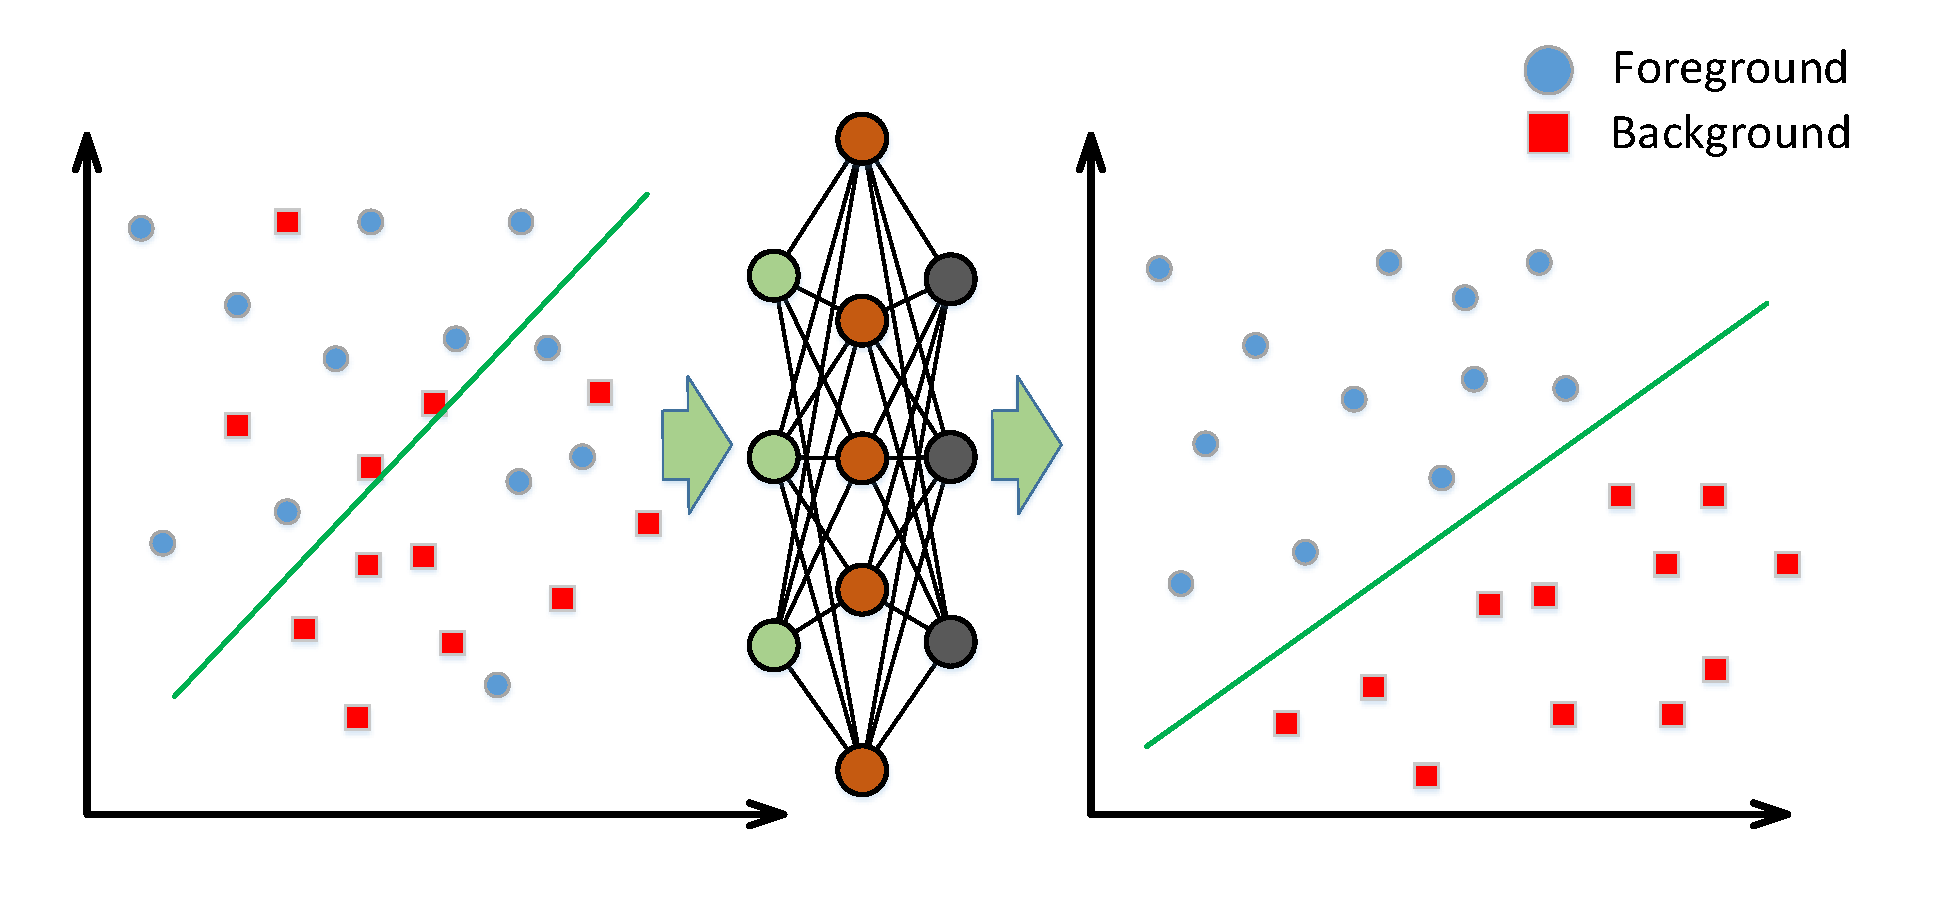
\includegraphics[width=\linewidth]{figure/fig1}
    % 图例里描述一下。
    \caption{It is hard to separate the foreground pixels from the background precisely in a time sequence.}
    \label{variation_chart}
\end{figure}


%图例解释困难点
To give an intuitive understanding of the pixel variations, we plot the historical observations and corresponding groundtruth of a single pixel in  \reffig{variation_chart}, with the X axis showing their range of variation and the Y axis representing the time. 
As we can see, there are several lines in three colors: blue, red and green. 
The blue one is called the pixel variation curve, which containing 100 original observations. 
Accordingly, the red one, the groundtruth curve is made of a piece of groundtruth data corresponding to the observations. 
The green one, which we call the transformed variation curve, is made of the outputs of the proposed approach. 
In practice, background subtraction is to produce a prediction curve, which is as near as possible to the groundtruth carve, by given the pixel variation carve. 

%传统方法的问题
Under ideal conditions like indoor videos, previous methods perform quite effectively, when distributions of background and foreground observations are remarkably different and the backgrounds are normally keeping static. 
While in fact, backgrounds can be rather turbulent and dynamic due to the complexity and diversity of nature scenes. 
Especially when illumination and camouflages are involved, background and foreground observations are easily confused and mixed up. 

%图例说明可能面临的挑战
For example, in \reffig{variation_chart}, it is noticeable that some foreground observations in blue line share the similarly value with background ones. 
In that case, those popular solutions will inevitably yield some sticky moments when separating the pixels in the blue line. 
Statistical methods, for instance, are no longer valid, because they only focus on establishing a statistical model for the background, while having little or no concern for the temporal coherence of these observations. 
Unfortunately, most previous methods, as far as we know, are not capable to take advantage of the temporal coherence of pixel variation. 
In other words, despite knowing that pixels from the background share some common patterns of variation in a temporal sequence, we still let the order information of sequential images all go to waste. 
%为了解决这些问题,我们必须利用好时序相关性
To alleviate this, order information of pixels must be taken in consideration. 
More concretely, we must find an efficient method to model the patterns of background pixels variations.


%variation transformation 介绍。
In this paper, a novel framework of pixel variation transformation are proposed. %用framework代替method?
Pixel observations are no longer considered independent of each other but regarded as a whole, which we call the pixel variation. 
Consequently, the classification of pixels can be viewed as a transformation of pixel variations, from the observation sequences to the prediction sequences. 
In the specific implementation, we trained a FCN to learn a transformation for the pixel variations by mapping them into a new space where it is close to the groundtruth, just like the green line in \reffig{variation_chart}. 
After thresholding, we can easily get the labels of each observation. 
%方法的好处是
The benefits from variation transformation are evident and clearly seen. 
It is hard to distinguish a foreground observation when its value are similar to the background ones. 
However, classification on the transformed variation is much convenient and intuitive, due to the advantage of temporal information. 
With the aid of deep learning method, the proposed approach can be effectively implemented.

% 公式表达
%And the definition of region searching method $G(x,y)$ is shown as follows:
%\begin{equation}
%    G(x,y) =  \mathop{\argmin}_{}{ \lVert I_t(m,n) - I_b(x,y) \rVert_{1}  } \quad  m,n \in x,y \pm R,
%\end{equation}

%where $x$ and $y$ is the location of pixels. And $I_t$ is the current frame, where $t$ is the
%time index.

%me
\section{BACKGROUND SUBTRACTION VIA DEEP VARIATION TRANSFORMATION}
\label{sec4}
In this section, we introduce the proposed approach that consists of a novel FCN network for background subtraction. 
We explain the details of the procedures of pixel matrixes, which is a specific form of the pixel variation, and the architecture of our network. 


The complete system is illustrated in \reffig{flow_chart}. 
Firstly, we temporally sample the input and ground truth images to generalize the pixel variations, and reshape them into fixed-size matrixes and feed them into the network with its spatial neighbors. 
After reassembling the matrixes into the complete output frame, it is post-processed, yielding the final segmentation of the respective video frame.
\begin{figure*}[!t] % FIGURE: figure/fig1 
\centering
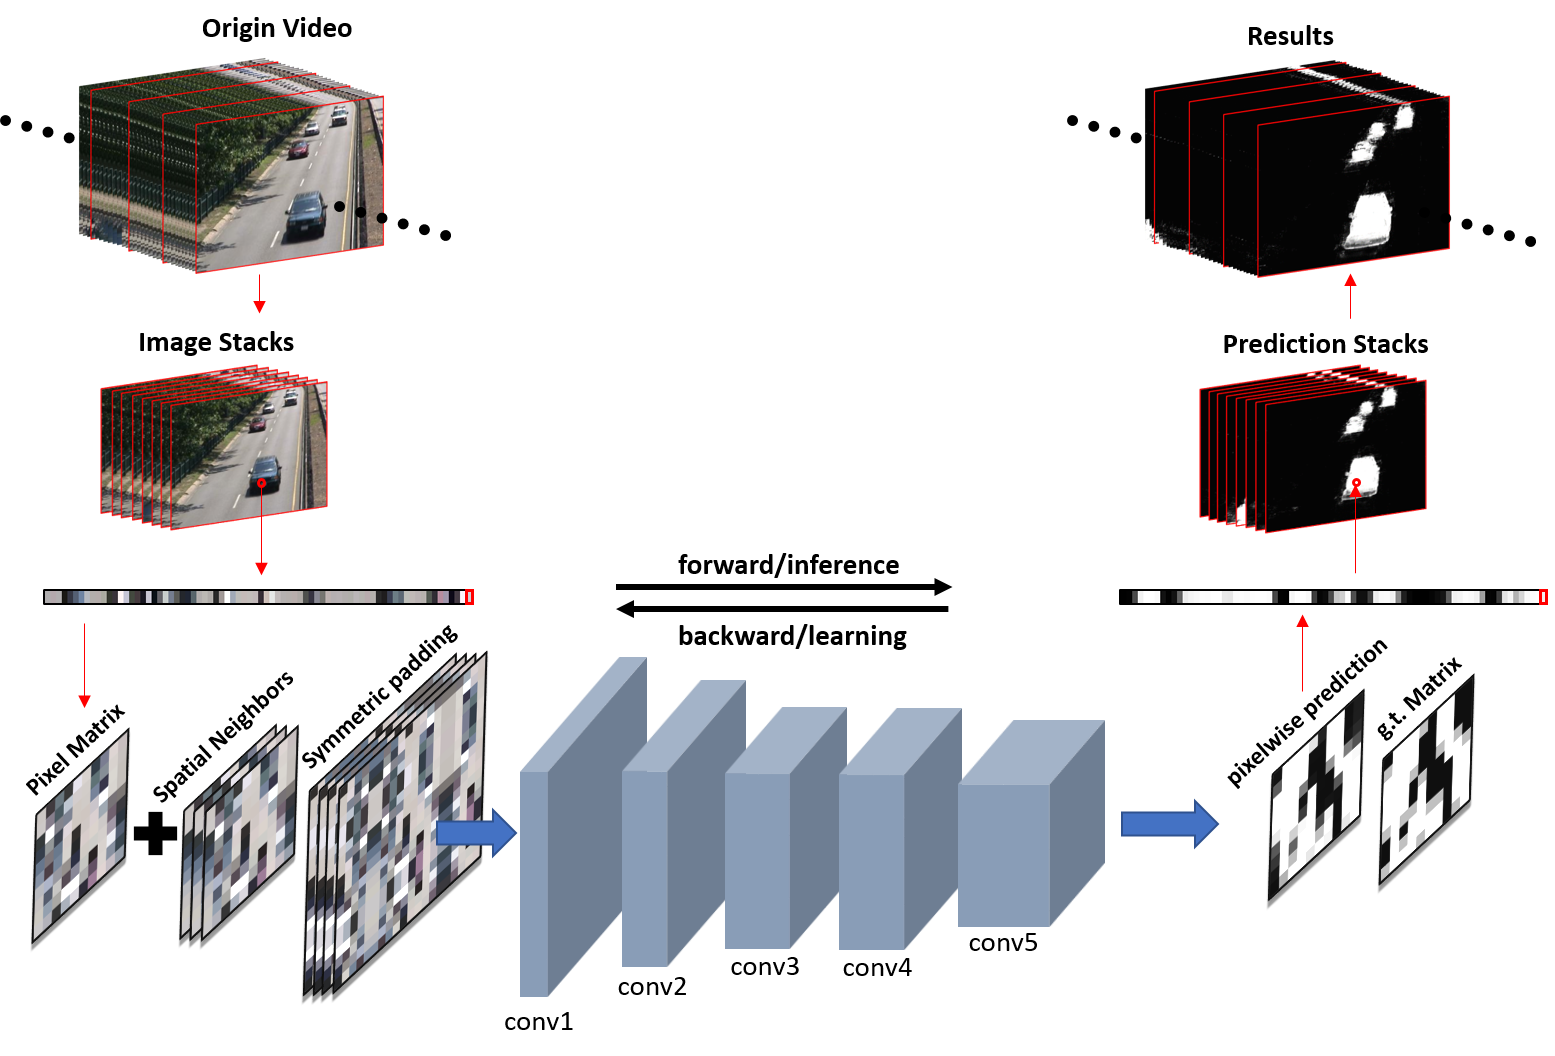
\includegraphics[width=\textwidth]{figure/fig2}
\DeclareGraphicsExtensions.
    \caption{Fully convolutional network can efficiently learn to make dense predictions for per-pixel tasks like semantic segmentation.}
    \label{flow_chart}
\end{figure*}


% 第一步是对原视频进行采样
Given different videos, the number of frames are generally different. 
However, the size of our input is fixed, which means a sampling processing is required to keep the length of pixel variations invariant. 
Therefore, image stacks are sampled form the given videos before the pixel variations are extracted. 
The given video and image stacks can be defined as follows: 
\begin{equation}
	Given \  Video=\{ I_1,I_2,I_3,\dots,I_L\} ,
\end{equation}

\begin{equation}
Stack_{(x)}=\{I_x,I_{(x+p)},I_{(x+2p)},\dots,I_L \},\quad p*l=L,\quad 1\leq   x\leq p , 
\end{equation}

% 解释采样的细节
Where $I_t$ represent the frame $t$ of the given video. 
And $p$ is an integer number depended on the video frames length. 
For each video, we can produce multiple image stacks and choose one of them for the training. 
In addition, thanks to the temporal sampling, we can get compact pixel historical observations containing more temporal information than the continuous pixel sequences. 
This works well when it comes to some situation where the moving objects keep stationary for a long time. 

% 第二步提取Pixel variation
In order to make use of the temporal information of pixel historical observations, we regard the sampled observations from a single pixel as a whole, namely the pixel variation. 
After the temporal sampling, a large number of observation sequences, or pixel variations, are extracted from the chosen stack, which is shown as follows:
\begin{equation}
Sq_{(m)}=\{P_1^m,P_2^m,P_3^m,\dots,P_n^m\},
\end{equation}

Where $P_t^m$ denotes the numerical value of pixel $m$ at frame $t$ in the chosen stack. 
Each of the pixel variation is a piece of temporal information which containing the changing patterns of background pixels. 
And each of them is of fixed length $n$. 
It is notable that observation sequences are extracted from individual pixel positions, which promises that sufficient training data can be obtained with only one image stack.

% 第三步变成矩阵形式,解释为什么要把variation 变形
Our intention is to provide an end-to-end transformation of pixel variations, based on the strong learning ability of FCNs. 
However, vectors are not appropriate for the network training and learning. 
Besides, we also hope the pixel observations can be interacted with their further compatriots in temporal sequence. 
Thus we reshape the variations into pixel matrixes as the input of our network. 
A sample of pixel matrix $H^m$ is like this:
\begin{equation}
H^m=P^m_{i+j*d}=\begin{bmatrix}
 P^m_1& P^m_2  &\dots  &P^m_d \\ 
\vdots &  &  &\vdots \\ 
 P^m_{1+(d-1)d}& \dots & \dots & P^m_n
\end{bmatrix},\quad d^2=n,
\end{equation}

Pixel variations are put into the $d\times d$ matrix according to the order of top to bottom and left to right. 
The parameter $i$ and $j$ represent the column and row respectively. 
And the parameter $n$ is the total frame length of a variation, as the same as the observation sequences. 
To put it from another way, the pixel matrix is just a specific form of the pixel variation. 
Although the observation matrix and the observation sequence belong to different forms of the pixel variation, they consist of the same components, and share the common temporal information from the pixel variation. 
Since the pixel sequences are extracted from individual pixels, a large number of pixel matrixes may be extracted from only a single image stack.

%第四步空间近邻随机采样。
It is generally accepted that neighboring background pixels share a similar temporal variation.
In other words, there are some clues hidden in pixels' spatial neighbors. 
In order to benefit from the spatial context, we concatenate the pixel matrix with 3 neighboring pixel matrixes, denoted as $SM_1$, $SM_2$ and $SM_3$ respectively.
They are randomly selected in 8 nearest neighbors. 
The input matrix of our network is defined as:
\begin{equation}
H = C(H^m, SM_1, SM_2, SM_3),
\end{equation}

Where $C$ represents the concatenating process on the third dimension.
And $H$ is the input matrix of our network, which size is $d\times d\times 4$.

In the previous steps, videos are broken down into pixel matrixes which contain abundant background information. 
Next, the groundtruth matrixes are obtained in the same way, except the concatenating process. 
Both of them are put into the network for the training. 
However, the size of the input will decreased in the forward computation. 
In order to make output the same size as input, we borrow the idea from Image Semantic Segmentation \cite{Shelhamer2017fcn}, padding the input matribxes before the training. 
After the forward computing, variations are transformed in a new space where they can be easily classified by thresholding. 
The transformed pixel variation is defined as:
\begin{equation}
H_p= \mathcal L (E_x (H)),
\end{equation}

Where, $H_p$ denotes the output of network, which we call the prediction matrix, the forward computation of network is represented by $\mathcal L$, and $E_x$ denotes the symmetric padding of pixel matrix where we have lost none of the pixel information to make the output $H_p$ the same size as the pixel matrix $H$. 
Another advantage of symmetric padding is that the order information still remains.

For the loss function, we choose the Sigmoid Cross Entropy (SCE), which are helpful to address the learning slowdown. 
The formulation is as follows:
\begin{equation}
    \begin{aligned}
        & \ell_{H_p, H_{gt}} =  \sum\limits_{x \in X, y \in Y}^{} H_{gt}(x,y) log(Sigmoid(H_p(x,y)))  \\
        & + (1 - H_{gt}(x,y)) log(1 - Sigmoid(H_p(x,y))) \\
        & Sigmoid(x) =\frac{1}{1+e^{-x}}\  ,
    \end{aligned}
\end{equation}

Where $H_{gt}$ denotes the groundtruth matrix which is given by the corresponding GT stack. 
The SCE is calculated between the transformed matrixes and the corresponding groundtruth matrixes. 
Boundaries of moving objects and pixels that out of the region of interest are ignored in the cost function.
Finally, we get the transformed variation through the FCN, which are easier for classification. 
We globally threshold the values for each observation in order to map them to $\{0,1\}$ . 
The threshold function is given by
\begin{equation}
    \label{piecewise_fg}
    g(x,y) =
 \begin{cases}
  1,  \quad x < y       \\
  0,  \quad otherwise   \\
\end{cases},
\end{equation}

\begin{equation}
M(x,y)=g(H_p,r) ,
\end{equation}

After the thresholding calculations, our experiment results show that a random initialized FCNs, trained end-to-end on feature learning can achieve the state-of-the-art without further machinery. 
And the major contribution is that we demonstrate the effectiveness of temporal information in background subtraction.

Here we make a detailed introduction to the deep learning model we used and explain why we choose it.

Different with CNNs, fully convolution neural network (FCN) utilize convolutional layers with $1*1$ kernels to take the place of fully connected layers, which largely resolves these above-mentioned problems. 
First and foremost, the size of outputs are adjustable in FCNs, which allows an end-to-end mapping of pixel observation sequences and network outputs on the time sequence. 
We hope to determine the label of a pixel through the comparison of its compatriot in time sequence. 
There is one more point I ought to touch on, that since the feature maps are no longer need to be converted into vectors, spatial information can be retained . 
The last but not the least, FCNs have been used in sematic segmentation and researchers found FCNs have a strong learning ability which won't lost to the traditional ones. 
Meanwhile, it's also a high efficient computation model. 


Based on above-mentioned factors, FCN is designed as the alternative network architecture in this paper. 
The structure of our FCN for background modeling is shown in \reffig{flow_chart}. 
The proposed FCN contains 5 convolutional layers, 2 pool layers and a convolutional layer which have a filter size of $1*1$. 
We use the Rectified Linear Unit (ReLU) as activation function after each convolutional layer and the Sigmoid function after the last fully connected layer. 
We do not use any other tricks in our network training and the experiment results prove that the proposed approach is feasible and very effective.


\section{Experiments}
\label{sec5}
In this section, we ran comprehensive experiments to evaluate the performance of the proposed approach on the CDnet 2014 benchmark\cite{CDN2014} and CAMO-UOW. 
The CDnet is the largest dataset for background subtraction so far as we are aware, containing 11 categories with several complexly challenging scenes, such as Dynamic Background, Camera Jitter, Shadow, Night Videos, PTZ and so on. 
The CAMO-UOW is another challenging benchmark which contains 10 high resolution videos. 
For each video, one or two persons appear in the scene with the clothes in the similar color as the background.

The proposed approach is compared with several existing traditional state-of-the-art background subtraction algorithms, including the IUTIS-5\cite{Bianco2017TEC}, the SuBSENSE\cite{St-Charles2015SuBSENSE}, the WeSamBE\cite{Jiang2017WeSamBE}, sharable GMM the SharedModel\cite{Chen2015SharedModel}, word-dictionaries-based method the PAWCS\cite{Charles2015PAWCS}, the SemanticBGS\cite{Braham2017Semantic}, the AAPSA\cite{RAMIREZALONSO2016990}, etc. 
Moreover, two deep learning based algorithms are also compared with the proposed approach, which include DeepBS\cite{Babaee2017deep}, and DBMF\cite{Yang2018DBMF}. 
All the results of compared algorithms are provided by authors.

During the comparison, the F-measure(Fm) has been used for evaluation. 
The Fm is a general international standard in background subtraction which measures the segmentation accuracy by considering both the recall and the precision. 
The definition of Fm is shown as follows:
\begin{equation}
Fm= \frac{2\times precision \times recall}{precision + recall} = \frac{2TP}{2TP+FN+FP},
\end{equation}
% 
% 
% \begin{equation}
%     F=\frac{precision \dot recall}{precision - recall}  = \frac{2TP}{2TP+FN+FP},
% \end{equation}
%

Where TP, FP, and FN are true positives, false positives, and false negatives respectively, computed in pixels of all test frames for each video. 


The quantitative and qualitative comparisons are shown in \reftab{tab1} and  \reffig{results_chart} respectively. 
Due to the paper length, several typical videos are selected for the qualitative comparisons as well as the discussion. 
In the dynamic background scene, the video "canoe" is a typically challenging video which includes a large area of water rippling. 
The main challenge comes from the dynamic background, in which it is so hard to describe the background by a single image. 
In this condition, since the traditional background subtraction method such as the SharedModel and the WeSamBE do not have the enough ability to describe the complex dynamically background, they are fail to detect the people on the boat, as shown in the \reffig{results_chart}. 
Besides, the detected moving objects of the SharedModel are not accurate in boundary due to the utilization of texture features. 
In contrast, benefited from the strong learning ability of Deep Learning network, the DeepBS successfully detected the people. 
Unfortunately, since the DeepBS ignores the fact that a single background is not enough to describe the dynamic background, even the deep learning based algorithm is suffering from the detection of the boat shape. 
In contrast, the proposed approach performed superior than others in this scene, since the essence of background subtraction is considered as a binary classification of pixels' observation in time sequence. 
Based on this insight, the FCN network focuses on learning the patterns of the pixel variation rather than a static background image, and proposed approach achieves promising performance in the canoe video.

\begin{figure*}[!t]	\centering
    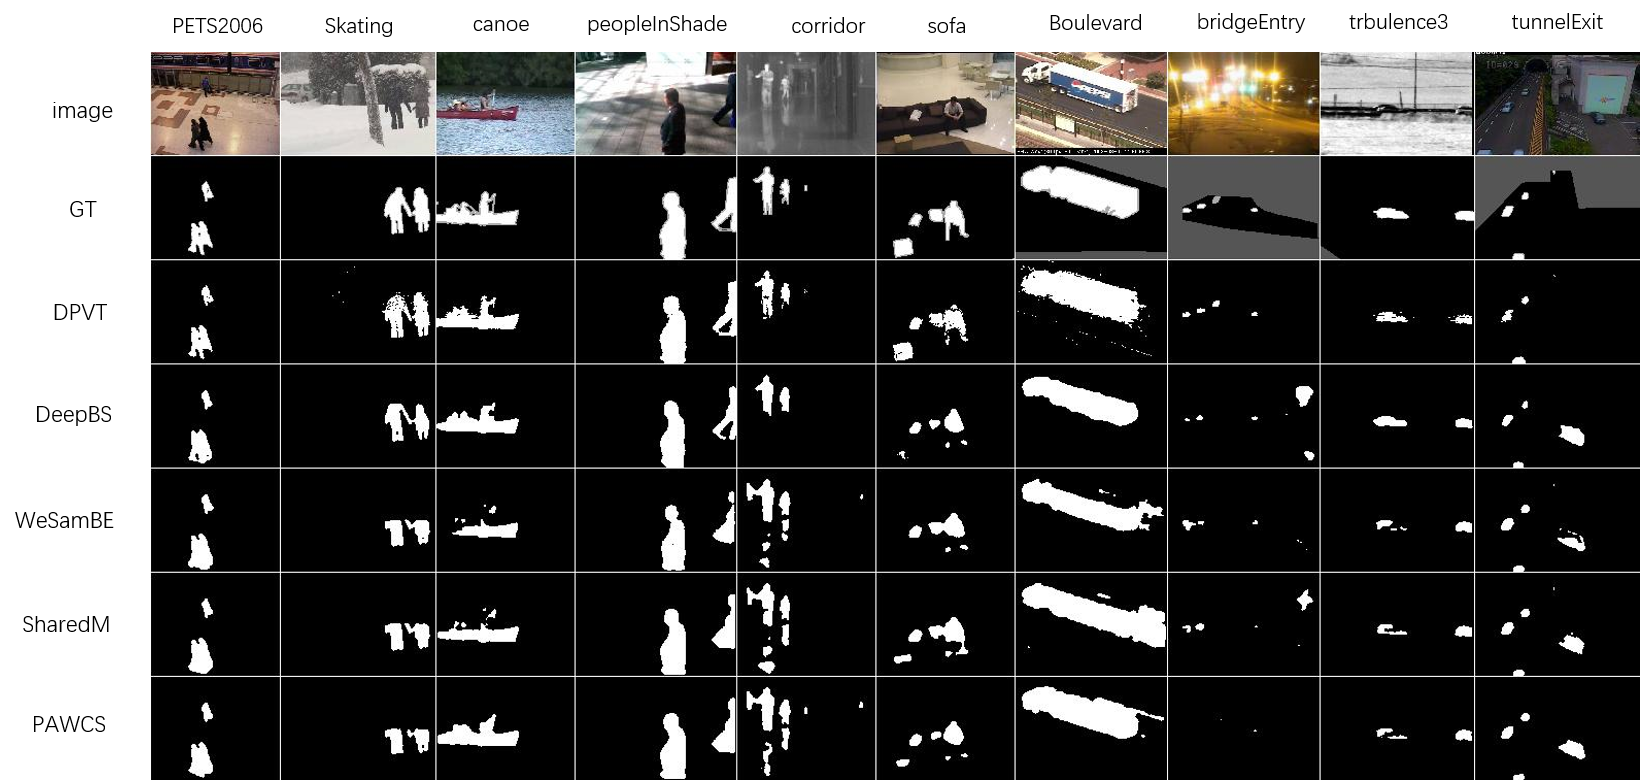
\includegraphics[width=\textwidth]{figure/fig3}
\DeclareGraphicsExtensions.
    \caption{The qualitative evaluation of the proposed method. All the results is followed in the CDnet 2014.}
    \label{results_chart}
\end{figure*}

As for the case of shadow scene, "peopleInShade" is a typical example with prevalent hard and soft shadows. 
In the traditional approaches, these shadow regions are usually segmented as foreground since it is also moving with the objects. 
Therefore, traditional methods like the PAWCS, the WeSamBE and the SharedModel falsely segments part of shadows as moving objects. 
In addition, the foreground provided by the UBSS is incomplete on the part of the pedestrian's body due to the interference of shades, which can be owing to the severe dependency of texture features. 
Whereas, the DeepBS performs well in this video benefited from the utilization of CNN. 
However, the shape of pedestrians are slightly deformed as the result of their matrix-wise processing of CNN. 
In contrast, derived from the fact that our DPVL focus on learning the pattern of pixels' variation in the shadow regions, proposed approach successfully segments the shadow part as the background and achieves the highest performance in the category of shadow scene.

In the video "corridor" among the Thermal scene, there is no color information since the videos are obtained through a Thermal camera. 
Moreover, the moving objects in these videos are exceedingly fuzzy and indistinct, which is the main challenge of this category. 
The WeSamBE, the SharedModel and the PAWCS successfully detect the target objects, owing to a stable background in this indoor video. 
However, they fail to remove the reflections since their modeling ability have already reached a limit under the extreme condition of thermal map. 
The DeepBS, by contrast, succeeds in eliminating most of the reflections. 
Meanwhile, the moving objects are also clearly divided from the background thanks to the strong modeling ability of CNN. 
However, due to the dependency of edge feature, a small object were missed in the detection result. 
Fortunately, the proposed approach focus on the pattern of pixels' variation, which should be theoretically effective even in the observation without the color information. 
Consequently, our DPVL performed much better than compared algorithms, with the situation that most parts of shadow are removed and the segmentation results are more accurate.

% \begin{table}[tab1]
\begin{table*}[!t]				% TABLE
\centering
\caption{The performance comparison of the proposed approach and some state-of-the-art algorithms on the video sequences from different categories in CDnet 2014.}
\label{tab1}
\begin{tabular}{lllllllllllll}
\hline
Videos      & baseline & dyna.bg & cam.jitter & int.obj.m & shadow & thermal & bad.weat & low f.rate & night vid. & PTZ    & turbul. & overall \\ \hline
DeepBS\cite{Babaee2017deep}      & 0.9580   & 0.8761  & \textbf{0.8990}     & 0.6097    & \textbf{0.9304} & 0.7583  & 0.8647   & 0.5900     & 0.6359     & 0.3306 & 0.8993  & 0.7458  \\
IUTIS-5\cite{Bianco2017TEC}     & 0.9567   & 0.8902  & 0.8332     & 0.7296    & 0.9084 & 0.8303  & 0.8289   & \textbf{0.7911}     & 0.5132     & 0.4703 & 0.8507  & 0.7717  \\
FTSG\cite{Wang2014FTSG}        & 0.9330   & 0.8792  & 0.7513     & 0.7891    & 0.8832 & 0.7768  & 0.8228   & 0.6259     & 0.5130     & 0.3241 & 0.7127  & 0.7283  \\
AAPSA\cite{RAMIREZALONSO2016990}       & 0.9183   & 0.6706  & 0.7207     & 0.5098    & 0.7953 & 0.7030  & 0.7742   & 0.4942     & 0.4161     & 0.3302 & 0.4643  & 0.6179  \\
CwisarDH\cite{Gregorio2014CwisarDH}    & 0.9145   & 0.8274  & 0.7886     & 0.5753    & 0.8581 & 0.7866  & 0.6837   & 0.6406     & 0.3735     & 0.3218 & 0.7227  & 0.6812  \\
PAWCS\cite{Charles2015PAWCS}       & 0.9397   & 0.8938  & 0.8137     & 0.7764    & 0.8934 & 0.8324  & 0.8059   & 0.6433     & 0.4171     & 0.4450 & 0.7667  & 0.7403  \\
SuBSENSE\cite{St-Charles2015SuBSENSE}    & 0.9503   & 0.8177  & 0.8152     & 0.6569    & 0.8986 & 0.8171  & 0.8594   & 0.6594     & 0.4918     & 0.3894 & 0.8423  & 0.7408  \\
SemanticBGS\cite{Braham2017Semantic} & 0.9604   & \textbf{0.9489}  & 0.8388     & 0.7878    & 0.9244 & 0.8219  & 0.8260   & 0.7888     & 0.5014     & 0.5673 & 0.6921  & 0.7892  \\
MBS\cite{Multimode_Background_Subtraction}         & 0.9287   & 0.7915  & 0.8367     & 0.7568    & 0.8262 & 0.8194  & 0.7980   & 0.6350     & 0.5158     & 0.5520 & 0.5858  & 0.7288  \\
WeSamBE\cite{2017_TCSVT_BG_7938679}     & 0.9413   & 0.7440  & 0.7976     & 0.7392    & 0.8999 & 0.7962  & 0.8608   & 0.6602     & 0.5929     & 0.3844 & 0.7737  & 0.7446  \\
ShareM\cite{2015_ICME_ShareModel}      & 0.9522   & 0.8222  & 0.8141     & 0.6727    & 0.8898 & 0.8319  & 0.8480   & 0.7286     & 0.5419     & 0.3860 & 0.7339  & 0.7474  \\
GMM\cite{Zivkovic2004}         & 0.8245   & 0.633   & 0.5969     & 0.5207    & 0.7370 & 0.6621  & 0.7380   & 0.5373     & 0.4097     & 0.1522 & 0.4663  & 0.5707  \\
RMoG\cite{Varadarajan2013}        & 0.7848   & 0.7352  & 0.7010     & 0.5431    & 0.7212 & 0.4788  & 0.6826   & 0.5312     & 0.4265     & 0.2470 & 0.4578  & 0.5735  \\ \hline
DPVTL        & \textbf{0.9757}   & 0.9303  & 0.8850     & \textbf{0.9322}    & 0.9274 & \textbf{0.9348}  & \textbf{0.8659}   & 0.7489     & \textbf{0.7529}     & \textbf{0.5836} & \textbf{0.9005}  & \textbf{0.8636} \\ \hline
\end{tabular}
\end{table*}

\begin{table*}[!t]
\centering
\caption{The performance comparison of the proposed approach and some classical methods and deep-based method DBMF .}
\label{tab2}
\begin{tabular}{llllllll}
\hline
Methods  & highway & office & Pedestrians & PETS2006 & Fall   & sofa   & overall \\ \hline
GMM\cite{Stauffer1999}      & 0.5788  & 0.2338 & 0.5202      & 0.6011   & 0.8026 & 0.5225 & 0.5432  \\
CodeBook\cite{WU2010739} & 0.8356  & 0.5939 & 0.7293      & 0.7808   & 0.3921 & 0.8149 & 0.6911  \\
ViBe\cite{Barnich2011_2011_TIP}     & 0.7535  & 0.6676 & 0.8367      & 0.6668   & 0.6829 & 0.4298 & 0.6729  \\
PBAS\cite{Hofmann2012Background}     & 0.8071  & 0.6839 & 0.7902      & 0.7280   & 0.3420 & 0.5768 & 0.6547  \\
P2M\cite{Yang2016P2M}      & 0.9160  & 0.3849 & 0.9121      & 0.7322   & 0.5819 & 0.4352 & 0.6604  \\
DBMF\cite{Yang2018DBMF}     & 0.9412  & 0.9236 & 0.8394      & 0.9059   & 0.8203 & 0.8645 & 0.8824  \\ \hline
DPVTL     & \textbf{0.9827}  & \textbf{0.9719} & \textbf{0.9729}      & \textbf{0.9753}   & \textbf{0.9269} & \textbf{0.9103} & \textbf{0.9567}  \\ \hline
\end{tabular}
\end{table*}

    
    \begin{table*}[!t]
\centering
\caption{The performance comparison of the proposed approach and some state-of-the-art algorithms on the video sequences from different categories in CAMO-UOW.}
\label{tab3}
\begin{tabular}{lllllllllll}
\hline
Methods  & MOG2\cite{ZIVKOVIC2006773} & FCI\cite{Baf2008FCI}  & LBA-SOM\cite{LBA-SOM2008} & PBAS & SuBSENSE & ML-BGS\cite{ML-BGS2007} & DECOLOR\cite{DECOLOR2013}       & COROLA\cite{SHAKERI201628} & FWFC\cite{Li2018CAMO}          & Ours          \\ \hline
Video 1  & 0.79 & 0.88 & 0.8     & 0.9  & 0.89     & 0.89   & 0.92          & 0.8    & \textbf{0.94} & \textbf{0.94} \\
Video 2  & 0.82 & 0.79 & 0.8     & 0.82 & 0.88     & 0.8    & 0.83          & 0.58   & 0.96          & \textbf{0.98} \\
Video 3  & 0.88 & 0.86 & 0.85    & 0.91 & 0.9      & 0.8    & 0.9           & 0.82   & \textbf{0.94} & \textbf{0.94} \\
Video 4  & 0.89 & 0.9  & 0.76    & 0.93 & 0.78     & 0.88   & 0.95          & 0.87   & 0.94          & \textbf{0.97} \\
Video 5  & 0.84 & 0.86 & 0.82    & 0.83 & 0.82     & 0.8    & 0.82          & 0.75   & 0.91          & \textbf{0.97} \\
Video 6  & 0.93 & 0.87 & 0.77    & 0.95 & 0.92     & 0.95   & \textbf{0.97} & 0.72   & 0.94          & 0.96          \\
Video 7  & 0.76 & 0.83 & 0.88    & 0.91 & 0.87     & 0.79   & 0.91          & 0.83   & 0.96          & \textbf{0.99} \\
Video 8  & 0.83 & 0.87 & 0.85    & 0.87 & 0.93     & 0.86   & 0.86          & 0.68   & 0.96          & \textbf{0.98} \\
Video 9  & 0.89 & 0.9  & 0.87    & 0.84 & 0.92     & 0.87   & 0.86          & 0.78   & 0.88          & \textbf{0.99} \\
Video 10 & 0.89 & 0.86 & 0.89    & 0.91 & 0.92     & 0.9    & 0.94          & 0.85   & 0.96          & \textbf{0.97} \\ \hline
average  & 0.85 & 0.86 & 0.83    & 0.89 & 0.88     & 0.85   & 0.90          & 0.77   & 0.94          & \textbf{0.97} \\ \hline
\end{tabular}
\end{table*}




The quantitative evaluation of proposed approach on CDnet 2014 is shown in the \reftab{tab1}. 
It can be inferred that the proposed approach significantly outperformed all of the compared state-of-the-art algorithms in most of complex scenes and achieved 6\% gain in FM over the second one on the whole dataset. 
Moreover, in order to compare proposed approach with the DBMF, which is also based on deep learning and only publish their results in several special vides. 
The proposed approach has also ran in these video and the results are shown in Table 2. 
Again, the proposed approach has noticeably better performance than the DBMF and some other classical background approaches.

	As shown in the \reftab{tab1} and \reftab{tab2}, previous deep learning based methods like the DeepBS and the DBMF achieve well performance. 
From our own perspective, that good performance should attribute to the stronger modeling ability and learning adaptation of CNN and FCN. 
However, the proposed approach focused on the pixels variation in temporal sequence rather than low-level static features such as color, edges and textures, which gives us the ability to avoid the shortcomings of the background models. 
Consequently, the proposed approach still get considerably better results, which over 10.46\% in FM metrics compared with the DeepBS and over 6.38\% compared with the DBMF.
The evaluation of proposed approach in CAMO-UOW dataset is shown in the \reftab{tab3}. 
Unlike the CDnet dataset, the videos of CAMO-UOW dataset are specially proposed for the moving objects with camouflage, which is the main challenge of this dataset. 
As shown in the \reftab{tab3} proposed approach achieves better performance compared to its competitions, with an average F-measure of 0.97, compared to values between 0.77 and 0.94 for the other methods. 
Therefore, it is fair to say that proposed approach performs better compared with their peers. 


In this dataset, target objects have the similar color and textures with the background, which brings a lot of difficulties and obstacles to traditional methods. 
However, our FCN is a powerful Neural Network model which is good at capturing the non-linearities of the manifold of pixel variations. 


All these experiments of the proposed method were implemented in matlab and ran on the computer with Nvidia tasela K80 GPU and all images are keep their original resolution. 
For each video in CDnet 2014, 100 training frames are extracted to produce the image matrix. 
It should be noted that the 100 frames only accounts for less than 10\% of total Groundtruth in CDnet 2014. 
In contrast, 90\% of data were used as training samples in the DBMF, which suggest that the proposed approach achieves well performance with limited training frames. 
Considering that the videos in CAMO-UOW have fewer frames, we reduce the number of training frames to 49. 
During the experience, the training set and testing set are completely separated. 
More specifically, our FCN network is random initialized. 
We train the network with mini-batches of size 100, a learning rate $α = 1 ∗ 10^{−3}$ over 20 epochs. 
The last threshold $R$ is set to 0.6.


% \begin{table}[!t]				% TABLE
%     \caption{The example of latex table}
% \label{tab_FBMS_nobk}
% \centering
%     \begin{tabular}{|l@{  }c@{  }c@{  }cc@{  }c@{  }c@{  }c|}
% \hline
%      \multirow{2}{*}{Videos} & \multicolumn{3}{c}{$\text{IFB}_{nobk}$} &  & \multicolumn{3}{c|}{IFB} \\
%     \cline{2-4} \cline{6-8}
%        & Re &Pr & Fm &  &  Re & Pr & Fm  \\
% \hline
% cats03          &   (\textbf{0.9472} ,\   &  0.5428 ,\  &   0.6901 )   &  &    (0.9063 ,\	 &  \textbf{0.7955} ,\	 &  \textbf{0.8473} )   \\
% bear01          &   (\textbf{0.9854} ,\   &  0.4806 ,\  &   0.6461 )   &  &    (0.8695 ,\	 &  \textbf{0.8673} ,\	 &  \textbf{0.8684} )   \\
% rabbits01       &   (\textbf{0.9530} ,\   &  0.4433 ,\  &   0.6051 )   &  &    (0.9510 ,\	 &  \textbf{0.8730} ,\	 &  \textbf{0.9103} )   \\
% cars5           &   (\textbf{0.9887} ,\   &  0.3693 ,\  &   0.5378 )   &  &    (0.9437 ,\	 &  \textbf{0.7108} ,\	 &  \textbf{0.8109} )   \\
% tennis          &   (\textbf{0.9364} ,\   &  0.4558 ,\  &   0.6132 )   &  &    (0.8808 ,\	 &  \textbf{0.7345} ,\	 &  \textbf{0.8010} )   \\
% farm01          &   (\textbf{0.9887} ,\   &  0.3897 ,\  &   0.5591 )   &  &    (0.8954 ,\	 &  \textbf{0.7462} ,\	 &  \textbf{0.8140} )   \\
% \hline                                                                                                           
% Average         &   (\textbf{0.9666} ,\   &  0.4469 ,\  &   0.6086 )   &  &    (0.9078 ,\    &  \textbf{0.7879} ,\   &  \textbf{0.8420} )   \\
% \hline
% \end{tabular}
% \end{table}

% Videos & GBSSP\cite{Lim2014_2014_ECCV} & calMoSeg\cite{2016_ECCV_Bideau2016}  & MLayer\cite{2017_ICCV_zhu2017multilayer}  & $\text{IFB}_{SU}$ & $\text{IFB}_{KA}$ & $\text{IFB}_{SI}$ & Videos & GBSSP\cite{Lim2014_2014_ECCV} & calMoSeg\cite{2016_ECCV_Bideau2016} & MLayer\cite{2017_ICCV_zhu2017multilayer}  &  $\text{IFB}_{SU}$ &  $\text{IFB}_{KA}$  &  $\text{IFB}_{SI}$  \\




\section{Conclusion}
\label{sec6}
In this paper, we proposed a noval background subtraction approach based on deep learning and the variation transformation learning. The DPVTL model include a FCN network and a noval variation transformation learing framework, which allows us to efficiently combine the temporal coherence and distribution information of pixels over a long period of time. Comparison with other traditional and deep learning methods shows that the DPVTL has good properties on several challenging scenes.
The future work will be focused on improving the DPVTL in terms of network architecture updating and integration of local spatial coherence.

% \section{Conclusions}
% In this paper,
% we proposed the IFB framework for background subtraction for the case of a freely moving camera.
% Unlike previous work in which attempts were made to improve the accuracy of the estimation of motion,
% our IFB focuses on integrating rough foreground and background cues for foreground segmentation.
% In particular, 
% foreground cues are detected by a GMM model with the estimation of background motion,
% while background cues are captured from spatio-temporal features filtered by homography transformation,
% where the SURF\cite{2006_SURF}, KAZE\cite{2012_KAZE}, SIFT\cite{lowe2004distinctive} features are used as examples.
% % the geometric constraints between the SIFT features.
% Then, super-pixels under multiple levels are utilized to integrate these cues.
% The efficiency of IFB results from the complementarity between foreground and background cues.
% The accuracy of the proposed approach is improved though the utilization of super-pixels under multiple levels.
% A comprehensive experiment to compare our results with the state-of-the-art shows the efficiency of our framework and points to its potential for use in practical applications.
% 
\ifCLASSOPTIONcaptionsoff
  \newpage
\fi

\bibliographystyle{IEEEtran}  
\bibliography{ref}  


\end{document}
